\section{Livello di trasporto}

\subsection{Introduzione e servizi a livello di trasporto}
Strumento che instaura una \textbf{connessione logica} tra i processi applicativi dei vari host, \textit{non è un collegamento fisico}.
Il \textbf{livello di trasporto} è in esecuzione sui \textbf{sistemi terminali}, non sui router. \newline
Durante l'invio scinde i messaggi in vari segmenti, passandoli al livello inferiore (livello di rete), mentre durante la ricezione riassembla il messaggio. \newline
Il \textbf{livello di rete} mette in comunicazione logica gli host. \newline
Il \textbf{livello di trasporto} è un \textbf{deamon} che mette in comunicazione logica i processi, usa i servizi del livello di rete, aspetta dal livello applicativo il messaggio da inviare e a chi inviarlo.

\subsubsection{Protocolli utilizzati}
I due protocolli utilizzati sono \textbf{TCP} e \textbf{UDP}. 
Il protocollo TCP offre vari servizi, tra cui: controllo di congestione e controllo di flusso, questo garantirà affidabilità ma avrà ritardi nel trasporto. \newline
Il protocollo UDP essendo non orientato alla connessione è meno affidabile, non avendo nemmno i controlli garantiti dal TCP, ma guadagna in velocità, non garantendo il corretto ordine di ricezione dei pacchetti e la ricezione di tutti i pacchetti. \newline
Entrambi i protocolli non garantiscono servizi di \textit{garanzia su ritardi} (visto che non possiamo prevedere il tempo di accodamento, il paccehtto potrebbe perdersi ed essere infinito bloccando tutta la connessione) e \textit{garanzia su ampiezza di banda}.

\subsection{Multiplexing e demultiplexing}
L'operazione di \textbf{multiplexing} è l'operazione di invio, prende i dati da inviare dai vari processi, incapsula il paccehtto con l'intestazione e invia il pacchetto, prende un pacchetto e lo divide in sottopacchetti.
L'operazione di \textbf{demultiplexing} è l'operazione di ricezione, prende i vari pacchetti, li ricompatta con le indicazioni dell'intestazioni e li manda alla \textbf{socket} (canale di comunicazione virtuale tra \textit{livello applicazione} e \textit{livello di trasporto}) corretta. \newline
Nell'intestazione a livello di trasporto abbiamo bisogno di minimo: l'etichetta numerica della socket associata ai processi di mittente e destinatario, quindi il numero porta d'origine e di destinazione, il resto dei campi dipende dal protocollo scelto. \newline
I protocolli \textbf{standard} hanno delle porte precise, motivo per cui già sappiamo qual è la porta di destinazione.
L'host usa gli indirizzi IP e i numeri di porta per inviare i vari segmenti. \newline

\subsubsection{demultiplexing senza connessione (UDP)}
Crea le socket con il numero di porta d'origine e di il numero di porta di destinazione. \newline
(da completare)

\subsubsection{demultiplexing orientato alla connessione (TCP)}
Crea le socket indentificata da 2 parametri sia per host mittente sia per host destinatario, un host può supportare più socket TCP contemporaneamente. \newline
Si possono creare thread web per gestire le socket, ogni thread del processo originale gestisce un client con una socket. 
La socket di benvenuto è la socket del server che attende la connessione dei vari client, una volta stabilita la connessione il client crea una socket con i suoi dati e i dati del server, infine il server crea una socket corretta con i dati suoi e del client, stabilendo la connessione tra i due host sulla socket appena creata. \newline
(da completare)

\subsection{Trasporto senza connessione: UDP}
Protocollo senza connessione, i segmenti (NON SONO DATAGRAMMI) UDP (User Datagram Protocol) possono essere perduti o consegnati in ordine errato. 
L'intestazione UDP è formato da numero porta orgine, numero porta di destinazione, lunghezza in byte del segmento UDP con intestazione e il checksum (aggiunge bit alla fine per controllare viene corrotto il pacchetto), tutti tasselli da 16 bit, totale di 8 Byte. 
UDP viene usato nei protocolli \textbf{DNS} e \textbf{SNMP}, viene utilizzato nelle applicazioni multimediali.

\subsubsection*{Checksum UDP}
Server a rilevare gli errori nel segmento trasmesso, controlla se ci sono bit alternati nella checksum confrontandolo con il checksum prima del trasporto. \newline
Operazioni del mittente:
\begin{itemize}
  \item Somma tutte le parole (tutti i campi presenti nel campo UDP, compreso di intestazione) tradotte in binari, nel caso in cui ci sia un riporto (17 bit) lo sommo al bit meno significativo, quindi il primo bit viene sommato al diciasettesimo bit, così che ora il pacchetto è lungo 16 bit. 
  \item La checksum è il complemento a 1 della somma (gli 1 diventano 0 e gli 0 diventano 1)
  \item Il client calcola il checksum e lo mette nell'intestazione
  \item L'host calcola il checksum e lo controlla con quello dentro l'intestazione, se rileva una discrepanza scarta il pacchetto
\end{itemize}
Errori multipli possono annullare bit corrotti, essendo somma binaria, se due bit opposti si corrompono il risultato non cambia.

\subsection{Principi del trasferimento dati affidabile}
Il servizio che offre il livello di trasporto è di un \textbf{canale affidabile}, ma l'implementazione del servizio utilizza un \textbf{canale inaffidabile} realizzato dal \textbf{livello di rete}, il livello di trasporto deve realizzare il collegamento e rendere affidabile il canale messo a disposizione dal livello di rete. \\
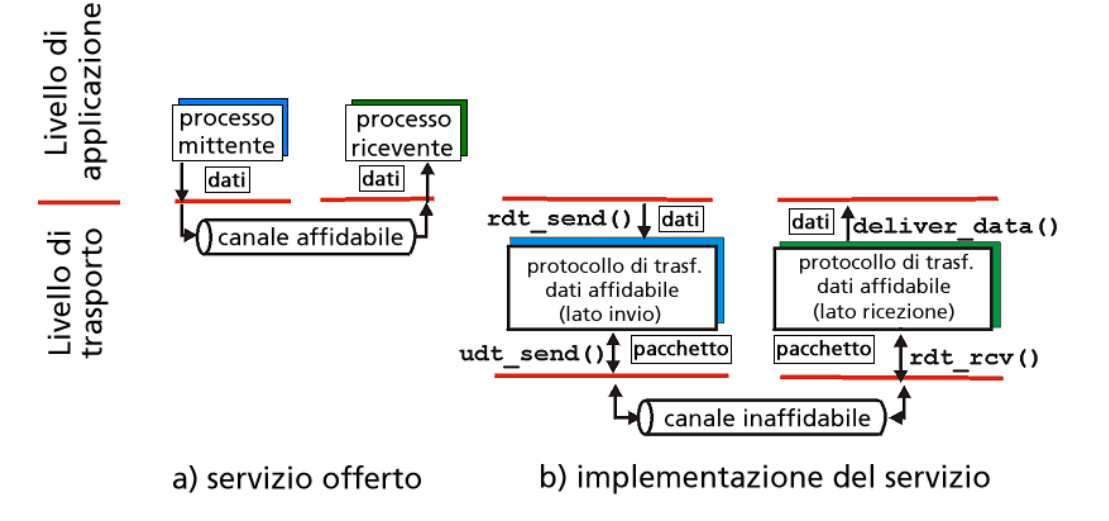
\includegraphics[width=\textwidth]{./img/implemntazionelivellotrasporto.png} \\

\subsubsection*{Rdt1.0: Mondo ideale}
In un mondo ideale dove il livello rete offre un \textbf{canale affidabile}, il livello di trasporto esegue solo queste operazioni:
\begin{itemize}
  \item L'host riceve i dati da inviare e il destinatario dal livello applicativo
  \item Crea i pacchetti da inviare
  \item Invia i dati al destinatario tramite il livello di rete
  \item \dots
  \item Il client riceve i dati dal livello di rete
  \item Estrae i dati 
  \item Invia i dati al livello applicativo
\end{itemize}

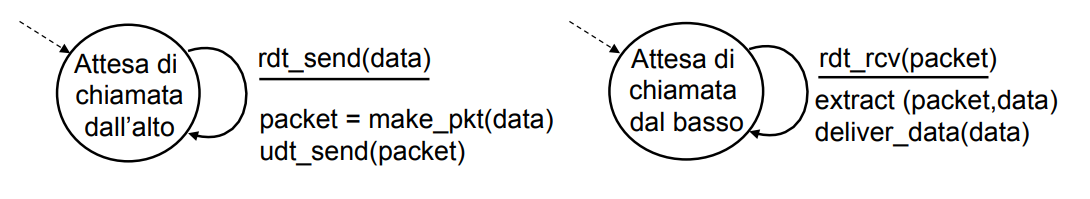
\includegraphics[width=\textwidth]{./img/rdt1.0.png} \\

\subsubsection*{Rdt2.0: canale con errori nei bit}
Il \textit{livello di trasporto} riceve i dati dal \textit{livello applicativo}, crea i pacchetti e aggiunge all'intestazione la checksum a ogni pacchetto. 
Invia il pacchetto al destinatario che ricalcolerà il checksum e controllerà se è corretto, nel caso in cui sia corretto manderà un messaggio di \textbf{ACK} (conferma di ricezione) al mittente e manderà il pacchetto al \textit{livello applicativo} del destinatario altrimenti manderà un messaggio di \textbf{NAK} (notifica pacchetto corrotto) al mittente che dovrà rimandare lo stesso pacchetto prima di procedere a inviare i restanti.

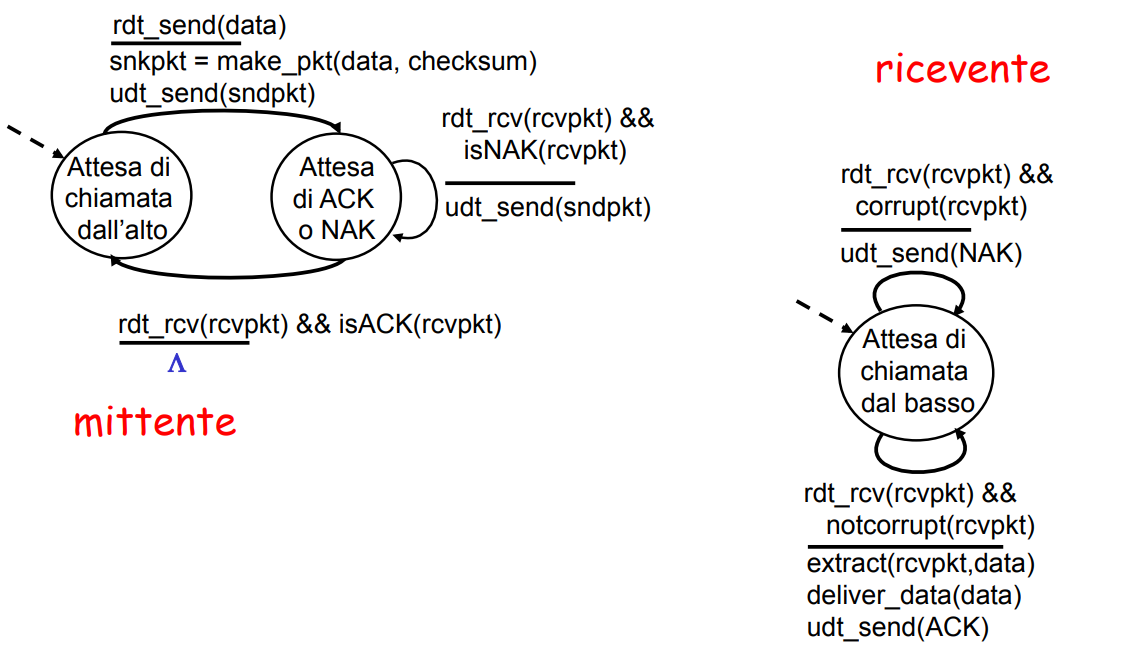
\includegraphics[width=\textwidth]{./img/rdt2.0.png} \\

\subsubsection*{Rdt2.1: il mittente gestisce gli ACK o NAK alterati}
Un problema di questo metodo è il caso in cui i pacchetti di \textit{ACK} o \textit{NAK} vengano corrotti, quindi il mittente non sa risposta corretta del destinatario, ritrasmettere è un opzione ma si possono essere dei \textbf{duplicati}. 
Dobbiamo risolvere il problema dei \textit{duplicati}, aggiungiamo il \textbf{numero di sequenza} a ogni pacchetto, quindi il ricevente scarterà il pacchetto duplicato nel caso in cui il mittente rimandi lo stesso capito anche avendo mandando un \textit{ACK} avendo già memorizzato il \textit{numero di sequenza}. \newline

Schema automa a stati finiti mittente: \newline
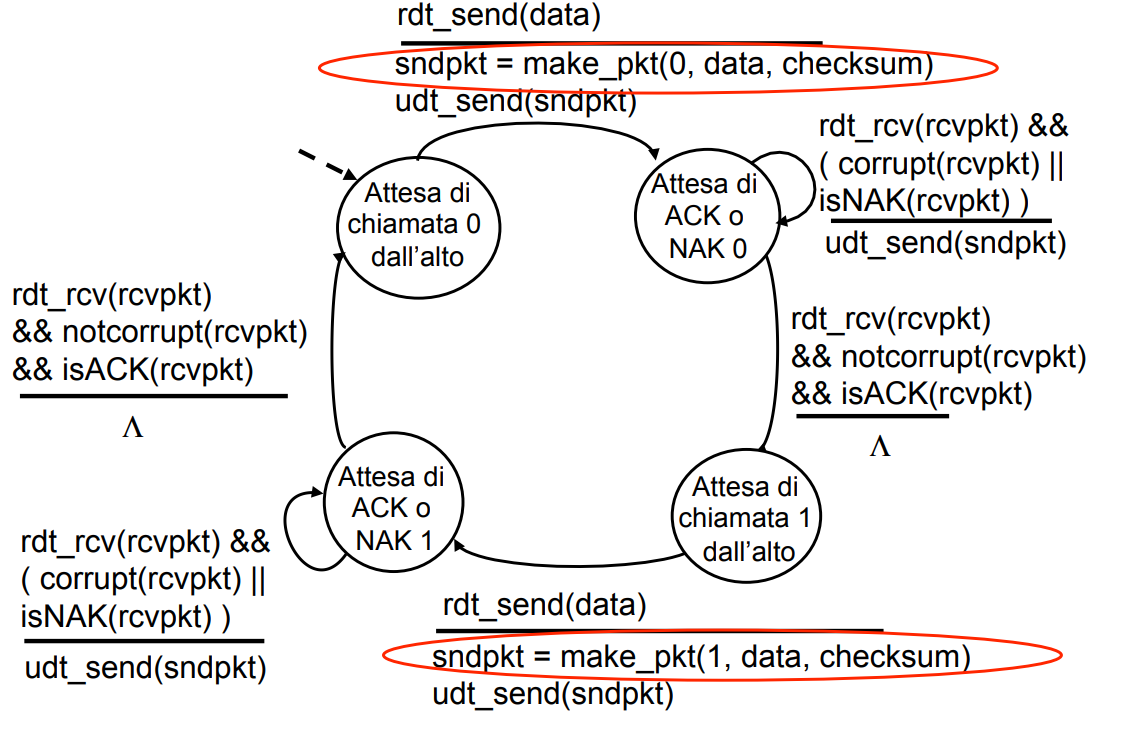
\includegraphics[width=\textwidth]{./img/rdt2.1mit.png}

Schema automa a stati finiti ricevente: \newline
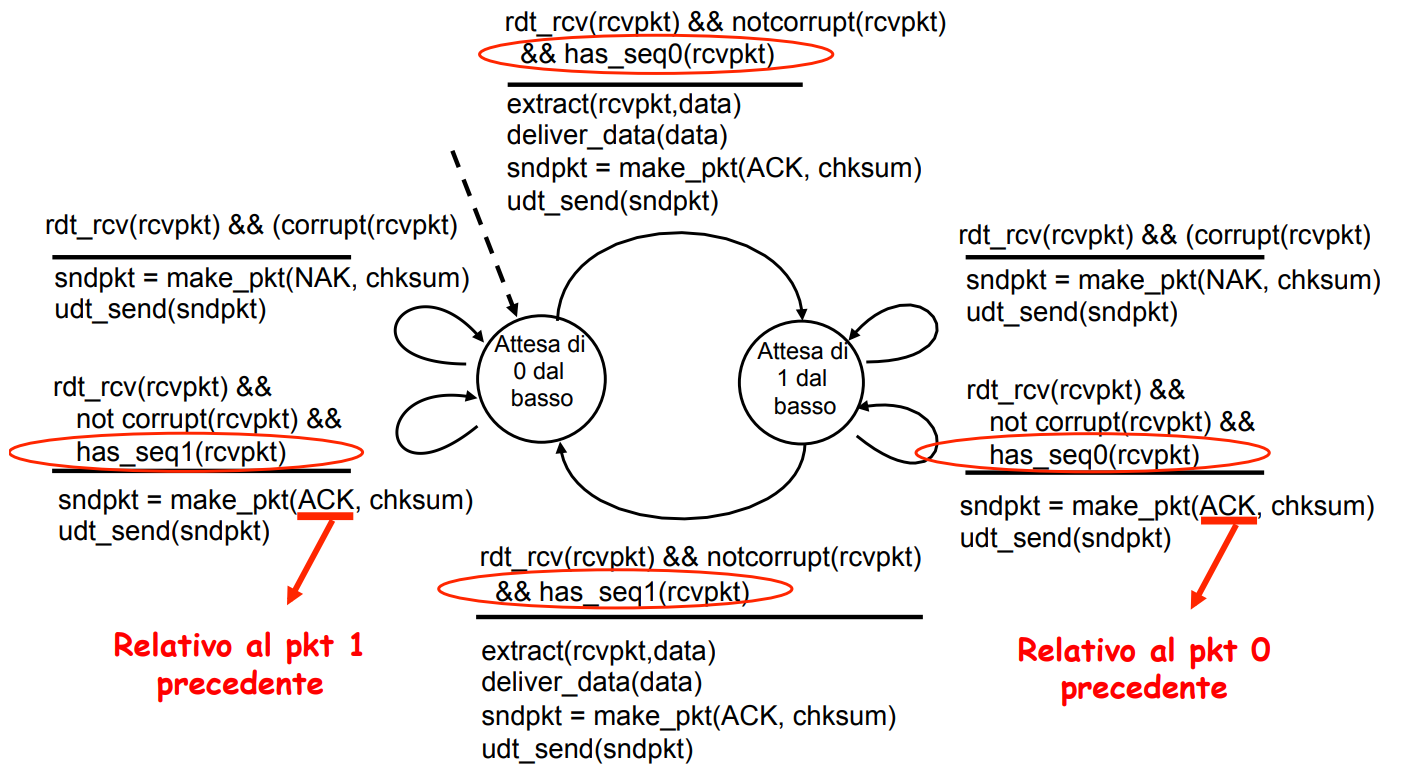
\includegraphics[width=\textwidth]{./img/rdt2.1ric.png}

\subsubsection*{RDT2.2: Protocollo senza NAK}
Si utilizza il numero di sequenza opposto al numero di sequenza del pacchetto che stiamo visualizzando come \textit{NAK}, se inivio il pacchetto con \textbf{numero di sequenza = 0} e il destinatario non capisce, manderà come messaggio un \textbf{ACK con numero di sequenza 1}, darà al mittente un ACK con un altro numero di sequenza come \textit{NAK}. \newline
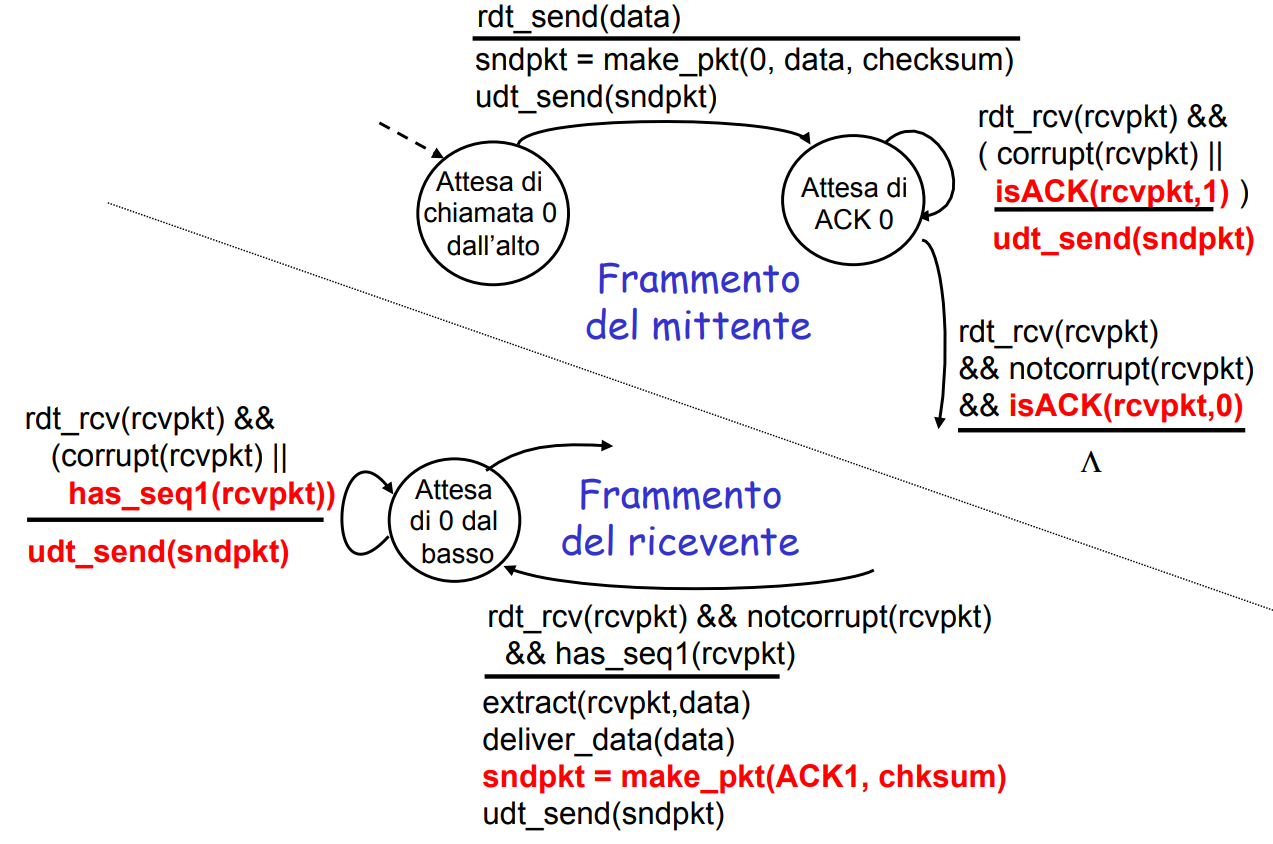
\includegraphics[width=\textwidth]{./img/rdt2.2nonak.png}

\subsubsection*{RDT3.0: canali con errori e perdite}
Si aggiunge un timer di attesa per la ricezione di un \textbf{ACK}, così in caso di pacchetto perso il mittente ritrasmetterà il pacchetto, nel caso in cui sia solo il ritardo il mittente invierà il pacchetto ma il duplicato verrà gestito tramite i numeri di sequenza. \newline 
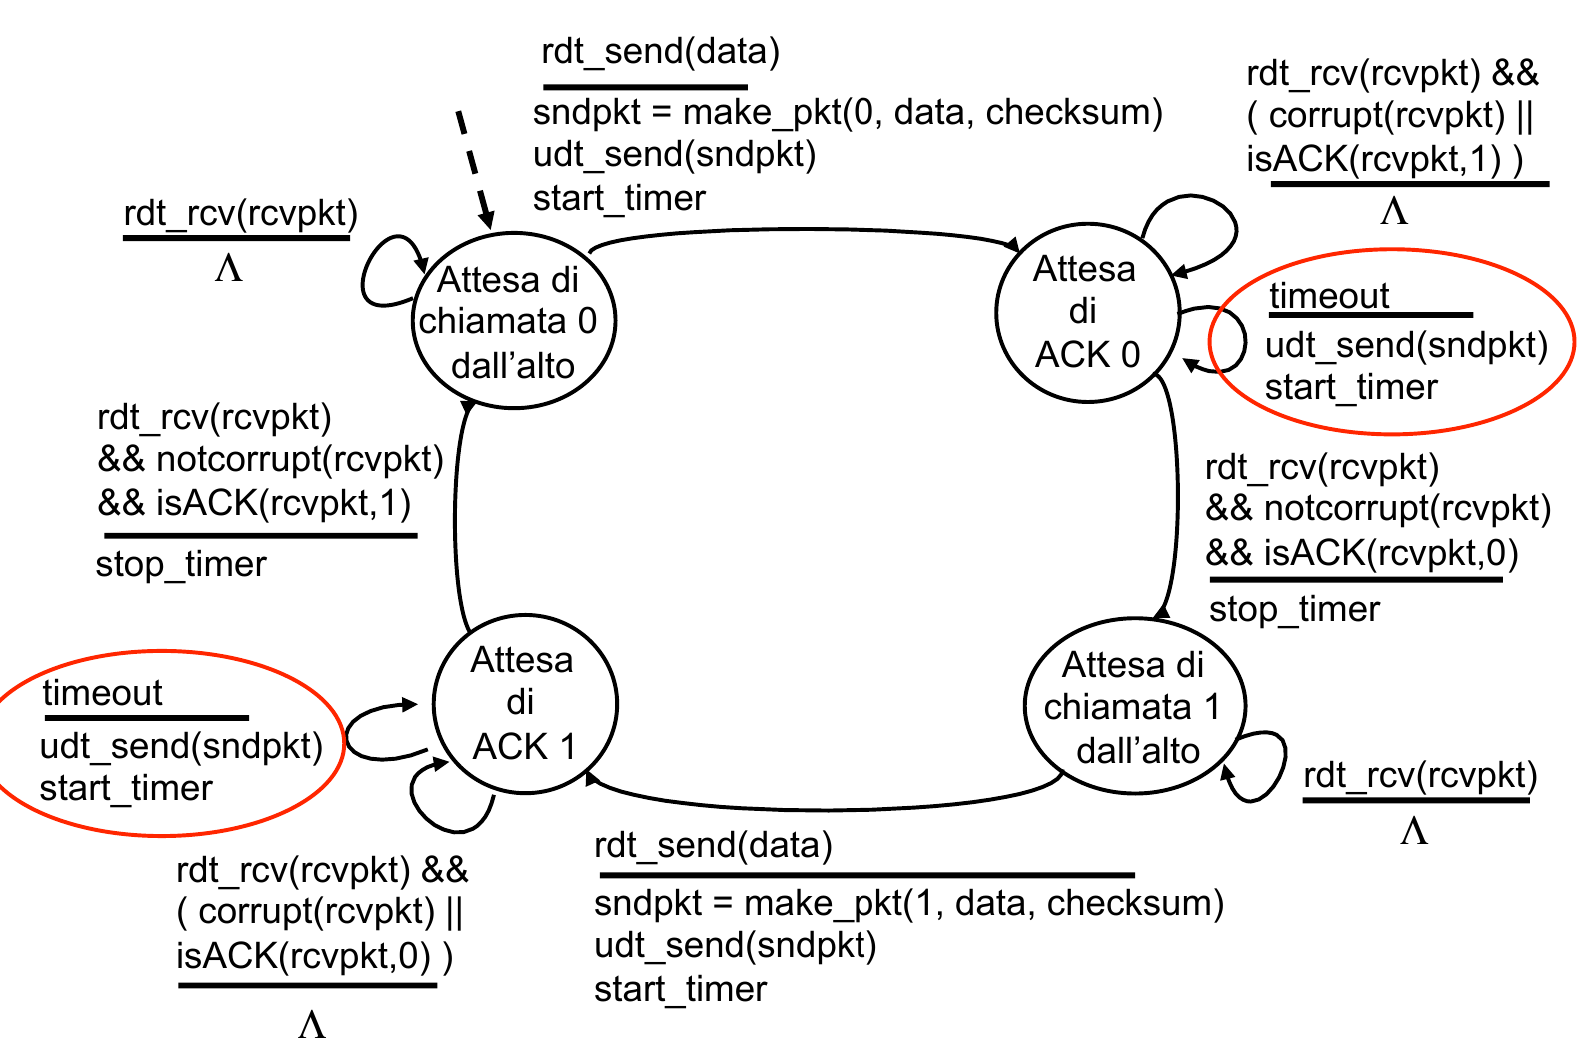
\includegraphics[width=\textwidth]{./img/rdt3.0mit.png} \newline
\begin{quote}
l'automa a stati finiti del ricevente è uguale a quello del \textbf{RTD2.2}
\end{quote}

\subsubsection*{RDT3.0: Perdita di pacchetto}
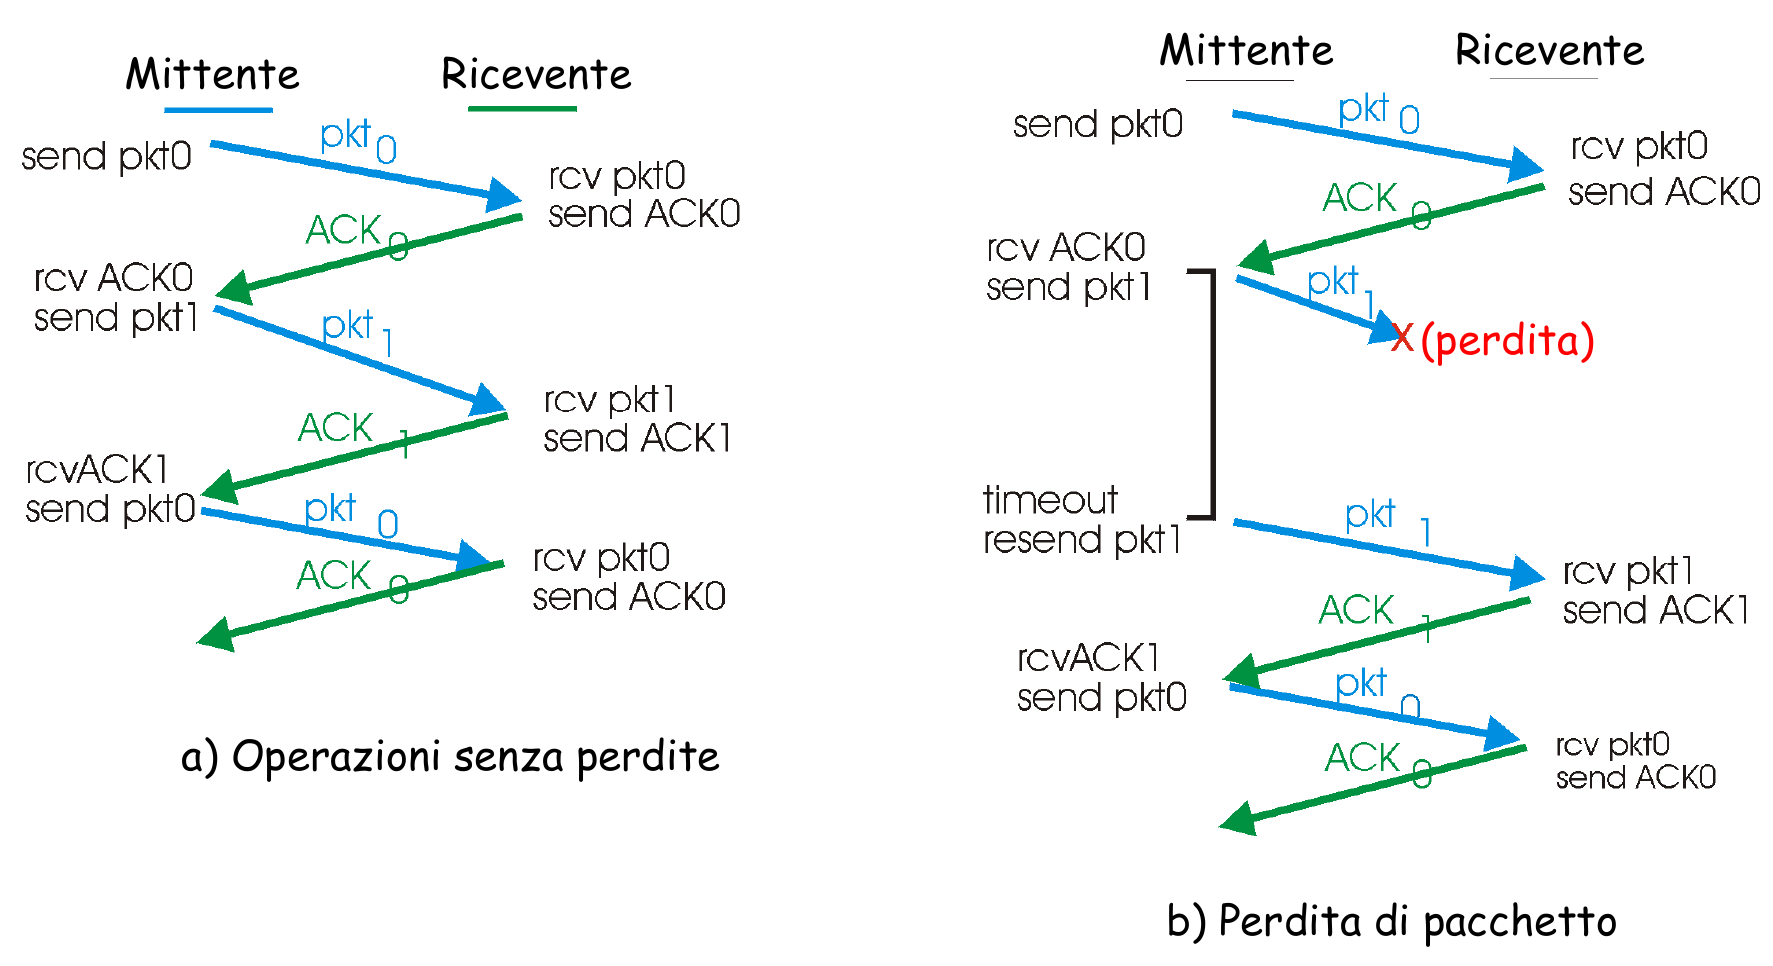
\includegraphics[width=\textwidth]{./img/rdt3.01.png} \newline

\subsubsection*{RDT3.0: Perdita di ACK}
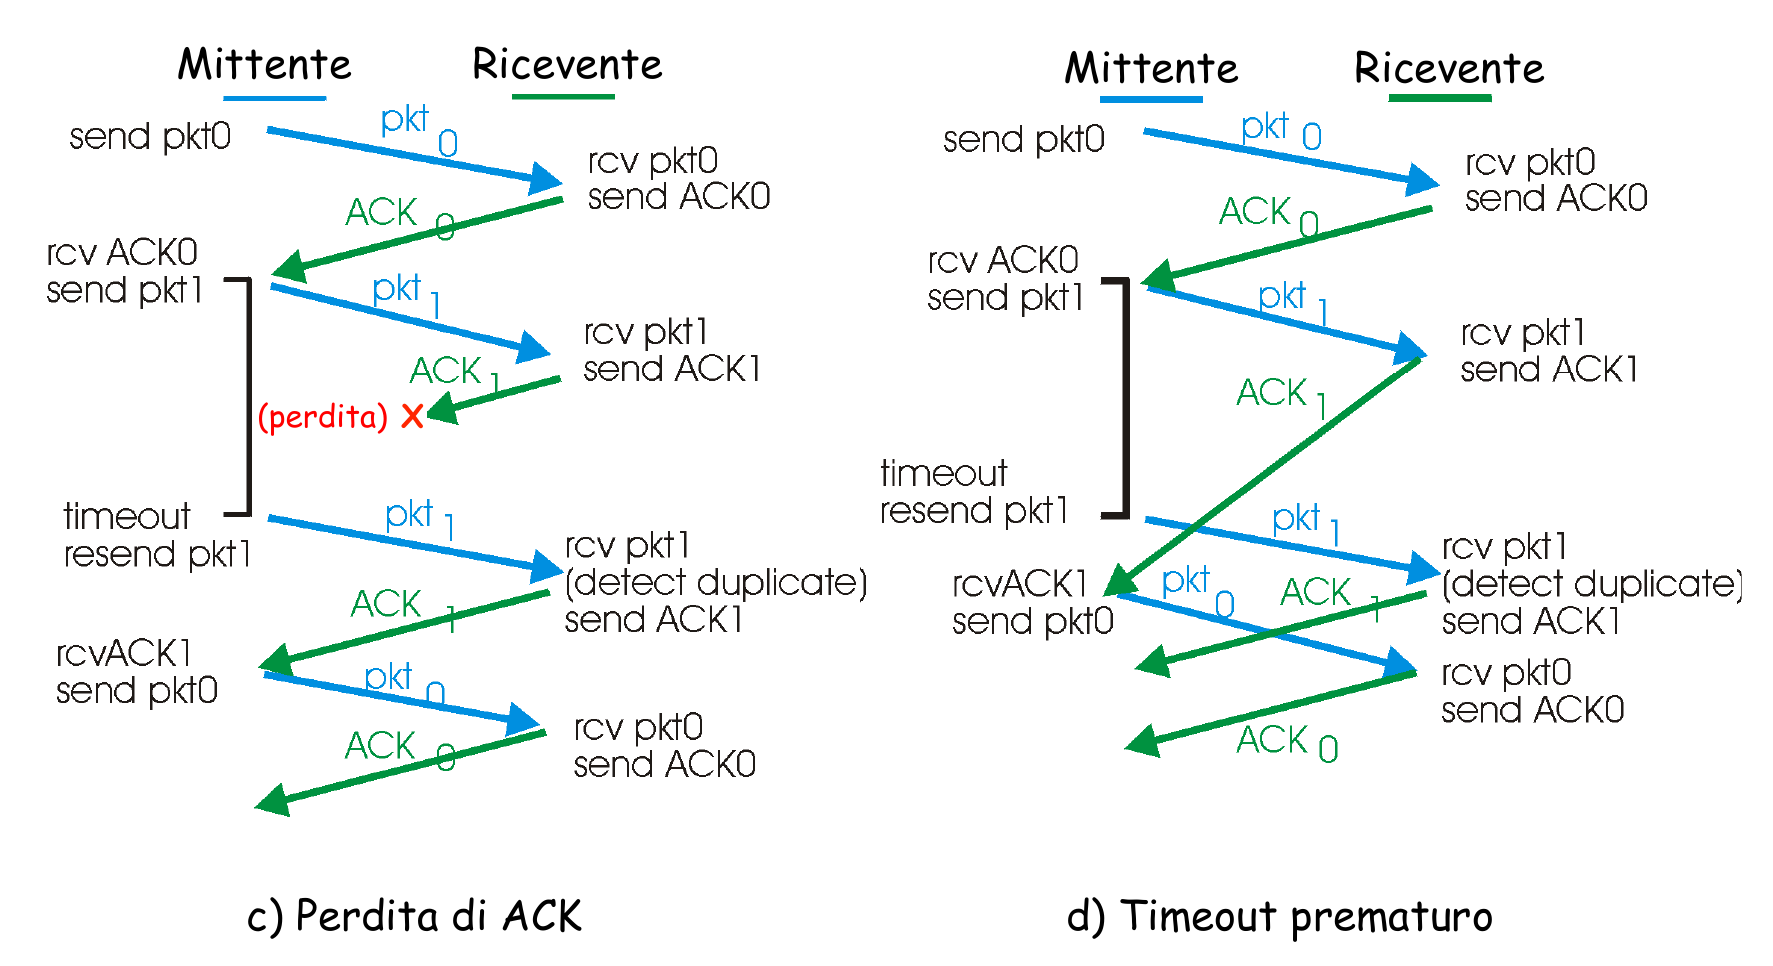
\includegraphics[width=\textwidth]{./img/rdt3.02.png} \newline

Il \textbf{RDT3.0} utilizza un algoritmo \textbf{STOP and WAIT} ma è molto lento, utilizziamo le \textbf{pipeline} per velocizzare il sistema. 

\subsubsection{Protocolli con pipeline}
Utilizzeremo due tipi di meccanismi, sono opposti come filosofia

\subsubsection*{Go-back-N}
\begin{itemize}
  \item Il mittente può avere fino a N pacchetti senza ACK in pipeline
  \item IL ricevente invia solo \textbf{ACK cumulativi}, non dà l'ACK di un pacchetto se c'è un gap
  \item Il mittente ha un timer per il più vecchio pacchetto senza ACK, se scade il time ritrasmette tutti i pacchetti senza ACK
\end{itemize}
L'ACK sarà con il numero di sequenza dell'ultimo pacchetto arrivato correttamente e in ordine, il mittente può continuare a mandare altri pacchetti, ma verranno rifiutati dal destinatario che manderà l'ACK con l'ultimo pacchetto arrivato oridinato. \newline
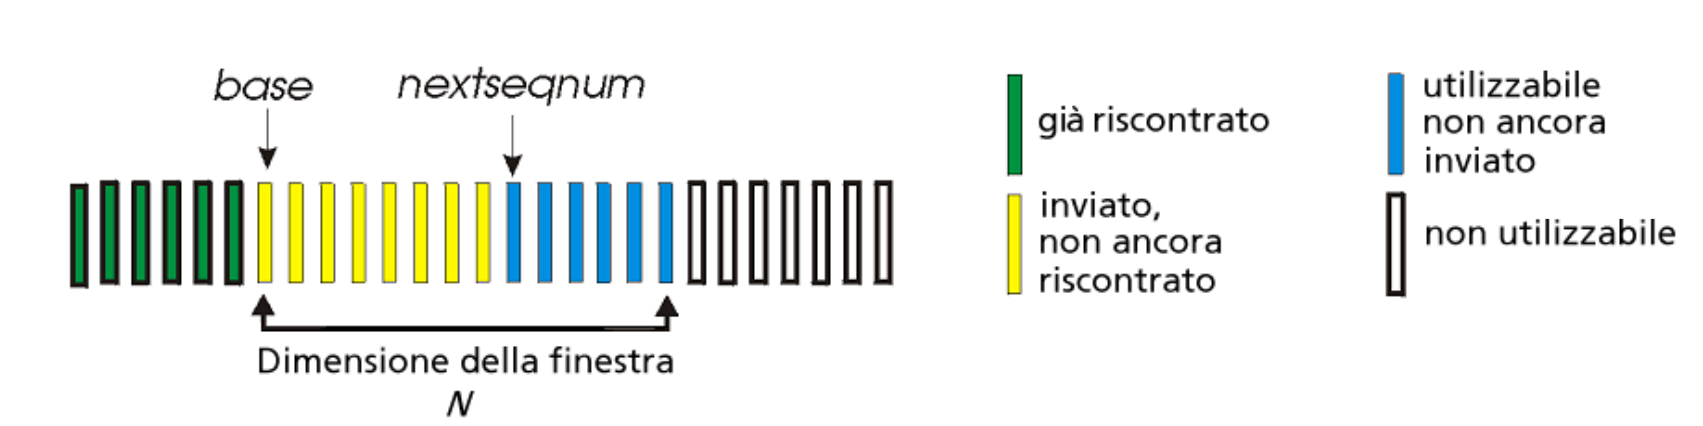
\includegraphics[width=\textwidth]{./img/gobackn.png} \newline
La finestra contiene N pacchetti inviati di cui ancora non è arrivato un riscontro.
nextseqnum: prossimo pacchetto da inviare

\subsubsection*{Selective repeat}
asd\newline
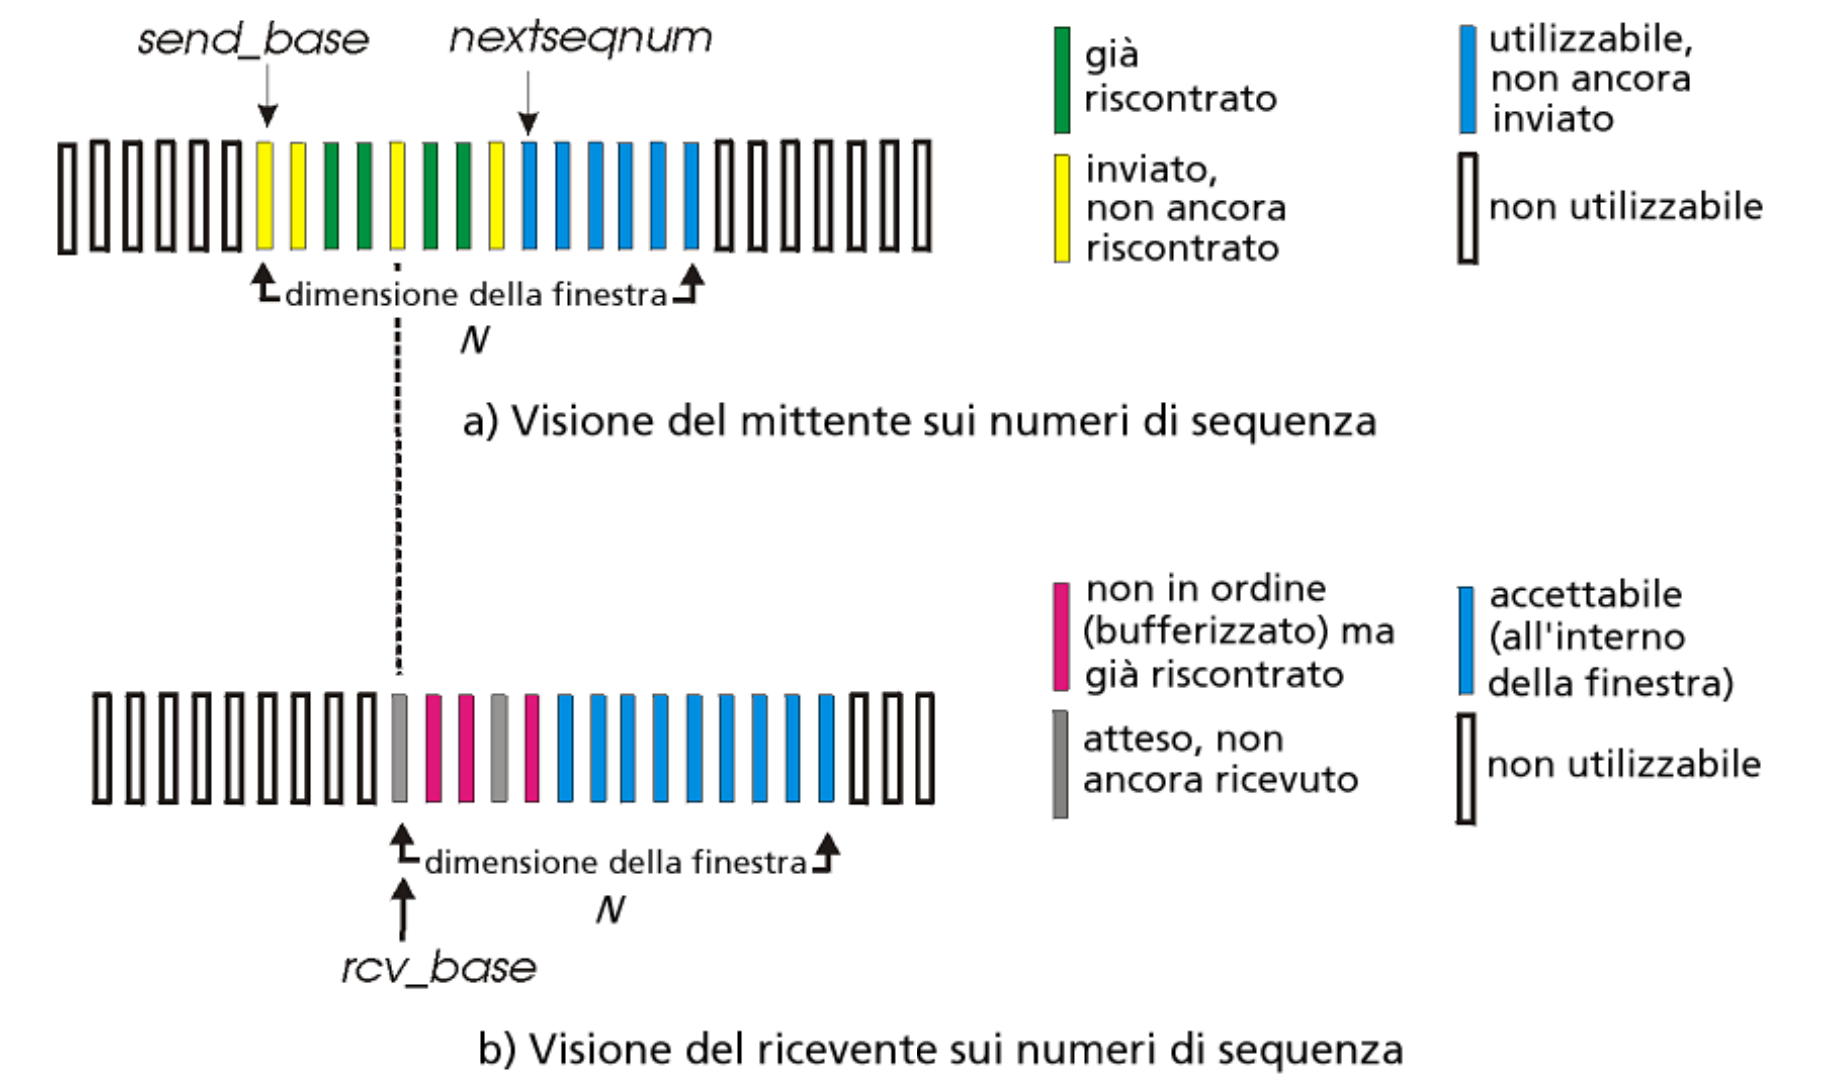
\includegraphics[width=\textwidth]{./img/ripetizioneselettiva.png} 

\textbf{THROUGHPUT}: tasso di occupazione medio con cui i dati vengono trasmessi sul collegamento, rapporto tra tutti i dati trasmessi (anche più volte) \\
\textbf{GOODPUT}: tasso con cui il livello applicativo di destinazione vede arrivare i dati utili, rapporto tra i dati utili e il tempo di trasmissione \\
Il \textit{throughput} è sempre maggiore del \textit{goodput}, solo nel caso ideale saranno uguale. 

\subsection{TCP: trasporto orientato alla connessione}
È un tipo di connesione \textbf{punto-punto}, tra mittente e destinatrio, \textbf{full duplex}, abbiamo un flusso di dati bidirezionale, e \textbf{orientato alla connessione}, \textit{handshaking a tre vie}, ha un flusso di byte affidabile, arrivano nella sequenza corretta. 
I dati vengono mandati in \textbf{pipeline}, attraverso un meccanismo \textit{sliding window}, abbiamo un \textbf{buffer d'inivio} e un \textbf{buffer di ricezione}, così che i paccehtti che arrivano fuori ordine vengono conservati e riordinati successivamente. 

\subsubsection{Struttura dei segmenti}
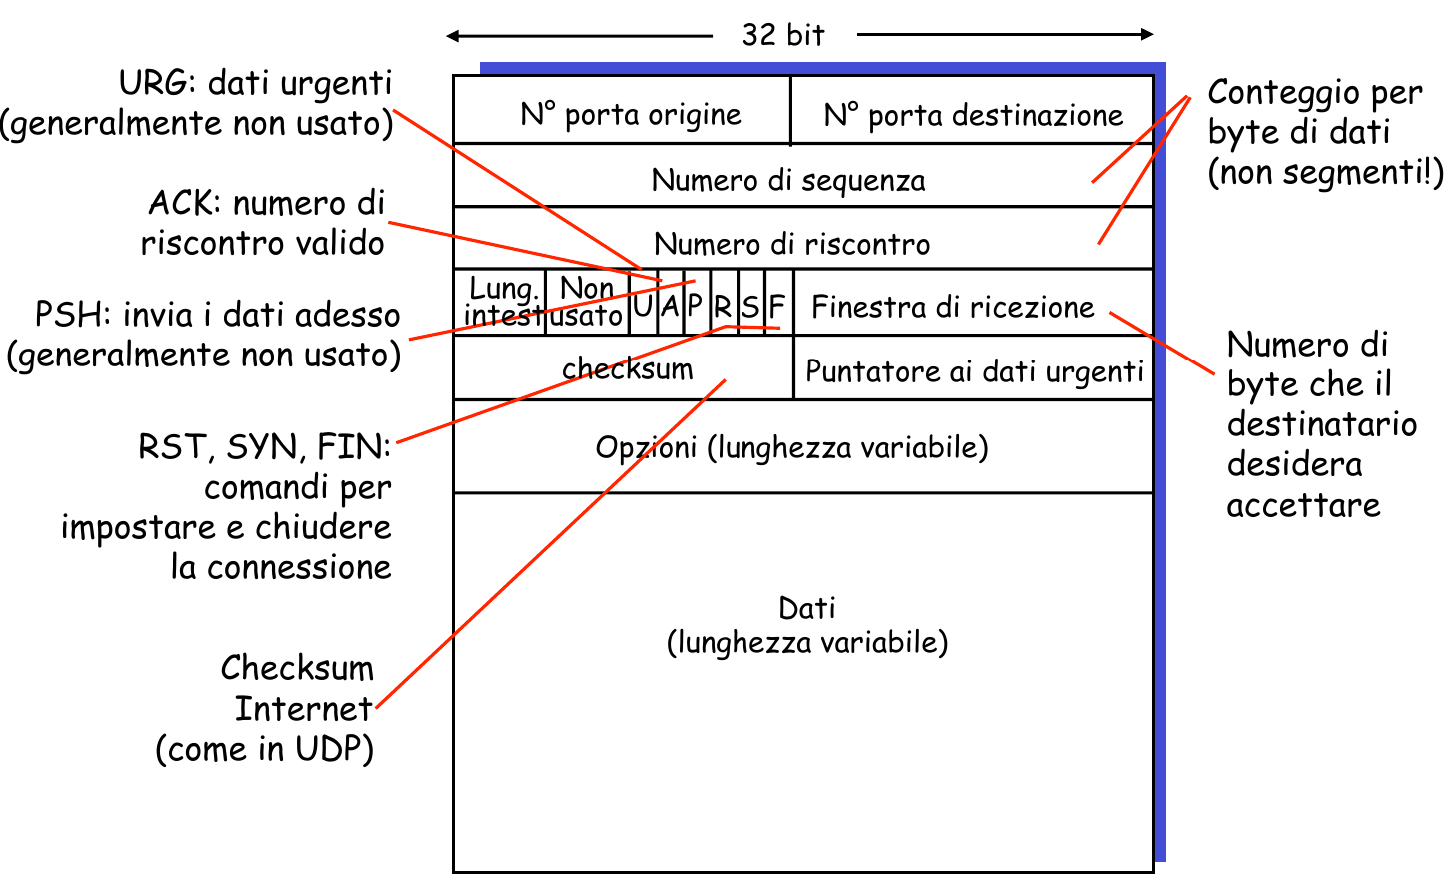
\includegraphics[width=\textwidth]{./img/segmento_tcp.png} 
\textbf{L'OVERHEAD} minimo del \textit{TCP} è di \textbf{20 Byte}. \\ 
\begin{itemize}
  \item Prima riga - uguale alla struttura del protocollo \textit{UDP}, serve per il multiplexing. 
  \item Seconda riga - \textbf{Numero di sequenza}: Posizione del primo Byte all'interno del payload (= MSS, Maximum Segment Size)
  \item Terza riga - \textbf{Numero di riscontro}: Il numero di riscontro sarà il primo byte del segmento successivo a quello arrivato
  \item Quarta riga - \textbf{BIT DI FLAG}: U (dati urgenti), A (\textbf{ACK}), P (PUSH), R (RST), S (SYN), F (FIN), gli ultimi tre sono comandi per impostare e chiudere la connessione 
  \item Quarta riga - \textbf{Lunghezza intestazione}: nel protocollo UDP è sempre 8 byte, qui no, verrà specificato pacchetto per pacchetto
  \item Quarta riga - \textbf{Finestra di ricezione}: Da non confondere con la \textit{sliding window}, dice quanto spazio si ha a disposizione per ricevere i dati 
  \item Quinta riga - \textbf{checksum}: grandezza di 16 bit, calcolata come la checksum dell'UDP
  \item Quinta riga - \textbf{Puntatore ai dati urgenti}: Nel caso in cui la flag U sia attiva ci sarà il puntatore alla memoria per quei dati
  \item Sesta riga - \textbf{Opzioni}: varie ed eventuali
\end{itemize}

\subsubsection{Gestione numeri di sequenza e riscontro del TCP}
Il \textit{numero di sequenza} è il primo byte del segmento nel payload, dipende dal mittente e da come gestisce la memoria del proprio \textbf{buffer di invio}. \\
Il \textit{numero di riscontro} utilizza un \textit{ACK cumulativo}, sarà il numero del prossimo dato che vuole ricevere in ordine, quindi sarà il primo byte del segmento che vorrà ricevere, quindi del successivo all'utltimo correttamente ricevuto e immagazzinato, dipende dal destinatario e da come gestisce la memoria del proprio \textbf{buffer di invio}. \\ 
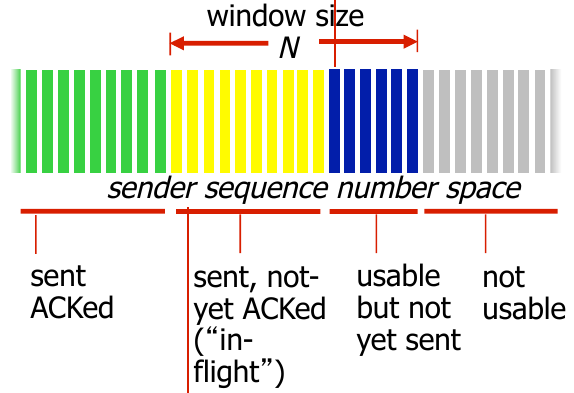
\includegraphics[width=\textwidth]{./img/tcpseqack.png} 

\subsubsection{Gestione del timer nel TCP}
Il problema principale è stimare correttamente la durata del timer utilizzando la \textbf{media mobile esponenziale ponderata}. La formula è la seguente:
\[
\text{EstimatedRTT}(t) = (1 - \alpha) \cdot \text{EstimatedRTT}(t-1) + \alpha \cdot \text{SampleRTT}(t)
\]
dove solitamente \(\alpha = 0.125\). \\
Bisogna calcolare la \textit{deviazione standard} del RTT:
\[
  \text{DevRTT}(t) = (1 - \beta) \cdot \text{DevRTT}(t-1) + \beta \cdot \lvert \text{SampleRTT} - \text{EstimatedRTT}\rvert
\]
dove solitamente \(\beta = 0.25\).
\[\text{TimeoutInterval} = \text{EstimatedRTT} + 4 \cdot \text{DevRTT}\]

\subsubsection{Trasferimento dati affidabile del TCP}
\subsubsection*{Eventi del mittente}
Crea un segmento con il numero di sequenza, sarà il primo byte del segmento nel payload, avvia il timer.
In caso di timeout o di \textit{ACK} duplicati, il protocollo TCP ritrasmetterà il pacchetto, riavvando il timer.
Controlla gli \textit{ACK} ricevuti, aggiorno ciò che è stato ricevuto e avvio il time nel caso in cui dovessi completare segmenti già inviati. 

\begin{lstlisting}
NextSeqNum = InitialSeqNum
SendBase = InitialSeqNum
loop (sempre) {
  switch (evento)

  evento: i dati ricevuti dall'applicazione superiore
    creano il segmento TCP con numero di sequenza NextSeqNum
    if (il timer attualmente non funziona)
      avvia il timer
    passa il segmento a IP
    NextSeqNum = NextSeqNum + lunghezza(dati)

  evento: timeout del timer
    ritrasmetti il segmento non ancora riscontrato con il piu' piccolo numero di sequenza
  
  evento: ACK ricevuto con valore del campo ACK y
    if (y > SendBase) {
      SendBase = y
      if (esistono timer non attualmente riscontrati)
        avvia timer
    }
} /* fine loop */
\end{lstlisting}
Quando si ritrasmette il pacchetto, il prodotocollo raddoppia il tempo di timeout al riavvio, nel caso di altra ritrassmissione raddoppierà il valore dell'ultimo timeout usato (quindi già raddoppiato).

\subsubsection*{Algoritmo della ritrassmissione rapida}
Quando si arriva a 3 ACK duplicati si effettua una ritrasmissione rapida, prima che scada il timer, il timer non viene spento.
Nel caso in cui nel frattempo sono arrivati i pacchetti successivi, il destinatario, al momento in cui riceverà il pacchetto che era andato perso e per cui ha mandato 3 ACK duplicati, invierà l'ACK del successivo dell'ultimo pacchetto ricevuto (sono stati bufferizzati nel mentre che aspettava quel pacchetto). 

\begin{lstlisting}
evento:  ACK ricevuto, con valore del campo ACK pari a y
  if (y > SendBase) {
    SendBase = y
  if (esistono attualmente segmenti non ancora riscontrati)
  avvia il timer
  } else {
    incrementa il numero di ACK duplicati ricevuti per y
    if (numero di ACK duplicati ricevuti per y = 3) {
      rispedisci il segmento con numero di sequenza y
  }
\end{lstlisting}

\subsubsection{Controllo del flusso}
Ricordiamoci che il protocollo \textit{TCP} inizializza delle zone di memoria per il \textit{buffer di ricezione} e \textit{buffer di invio}, il mittente non deve sovraccaricare il buffer del destinatario. 
Mittente e destinatario comunicano continuante quanto spazio hanno libero nei vari buffer.
Il valore di \textbf{RcvWindow} verrà inserito all'interno dei segmenti, il mittente limita i dati non riscontati \textit{RcvWindow}, così che non vengano inviati dati che verranno sicuramente persi. 
\textbf{RcvBuffer} funzione per la creazione della socket. \\ 
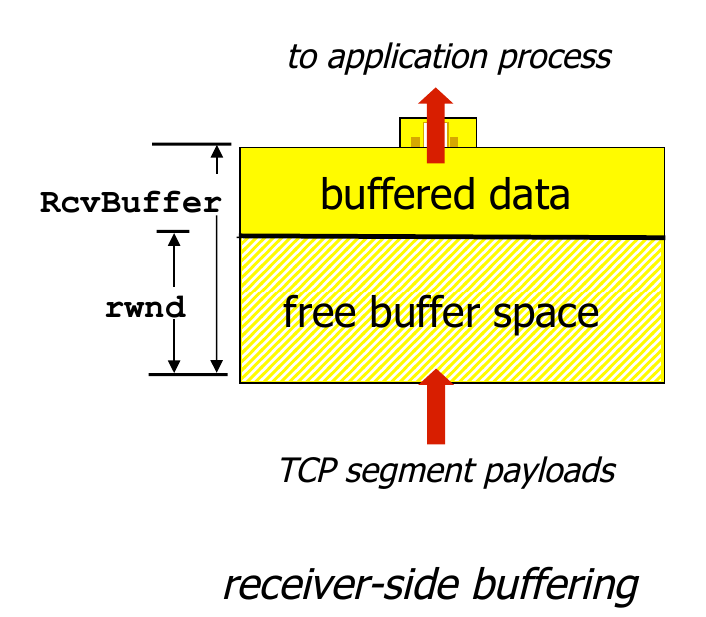
\includegraphics[width=\textwidth]{./img/tcpflowcontrol.png}  

\subsubsection*{Gestione della connessione: Handshake a tre vie}
Si stabilisce una connessione tra mittente e destinatario, si mettono d'accordo e inizializzano dei dati come \textit{numero di sequenza} e i \textit{buffer}. 
L'inizializzazione della connessione avviene tramite l'\textbf{Handshake a tre vie}:
\begin{itemize}
  \item Passo 1: il client invia un segmento SYN al server \\
      specifica il numero di sequenza iniziale \\ 
      nessun dato
  \item Passo 2:  il server riceve SYN e risponde con un segmento SYNACK \\
      il server alloca i buffer \\
      specifica il numero di sequenza iniziale del server
  \item Passo 3:  il client riceve SYNACK e risponde con un segmento ACK, che può contenere dati
\end{itemize}
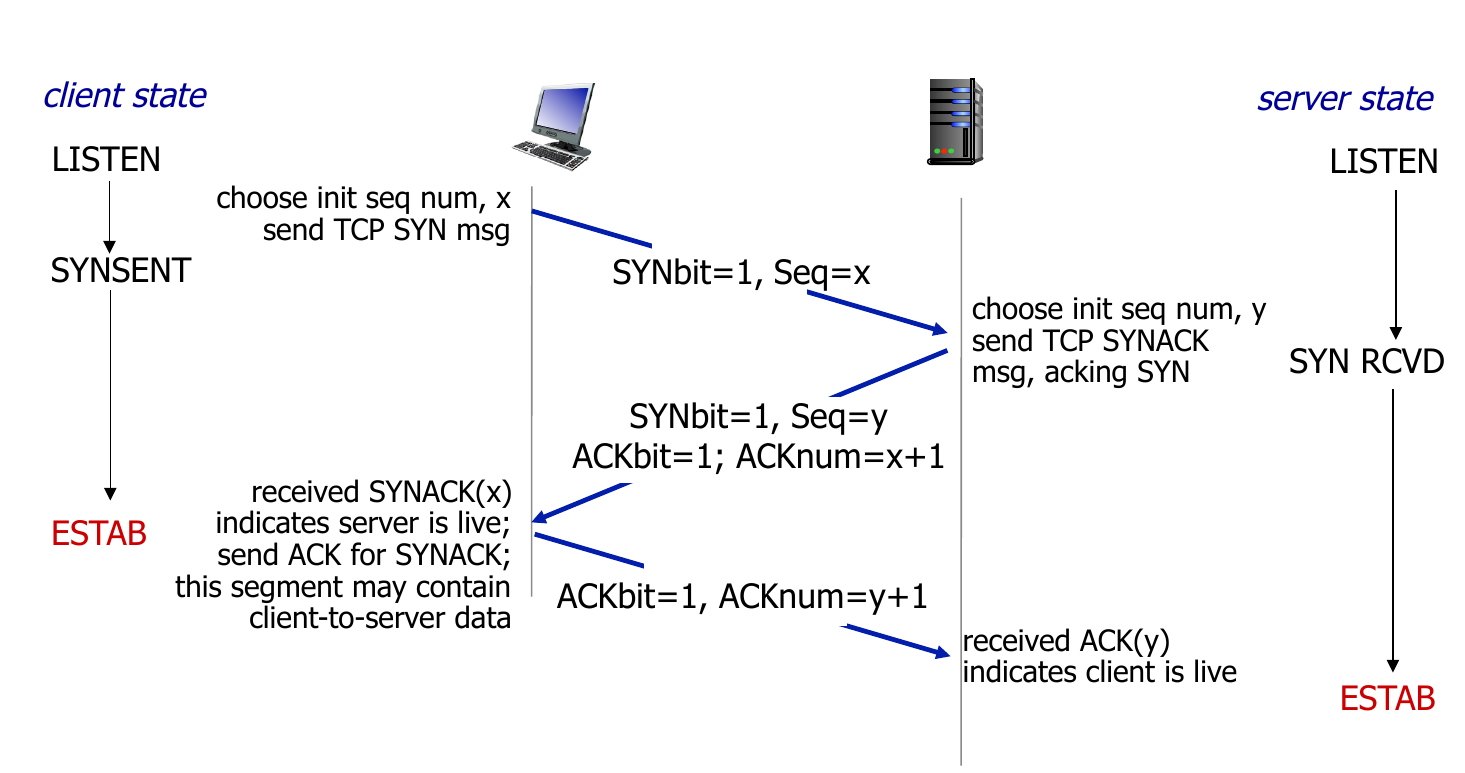
\includegraphics[width=\textwidth]{./img/handshake3vie.png} \\ 

Per chiudere una connessione abbiamo 4 passi: 
\begin{itemize}
  \item Passo 1: il \textit{client} invia un segmento di controllo FIN al server.
\item Passo 2: il \textit{server} riceve il segmento FIN e risponde con un ACK e invia un FIN.
\item Passo 3: il \textit{client} riceve FIN e risponde con un ACK. inizia l’attesa temporizzata - risponde con un ACK ai FIN che riceve 
\item Passo 4: il \textit{server} riceve un ACK. La connessione viene chiusa.
\end{itemize}
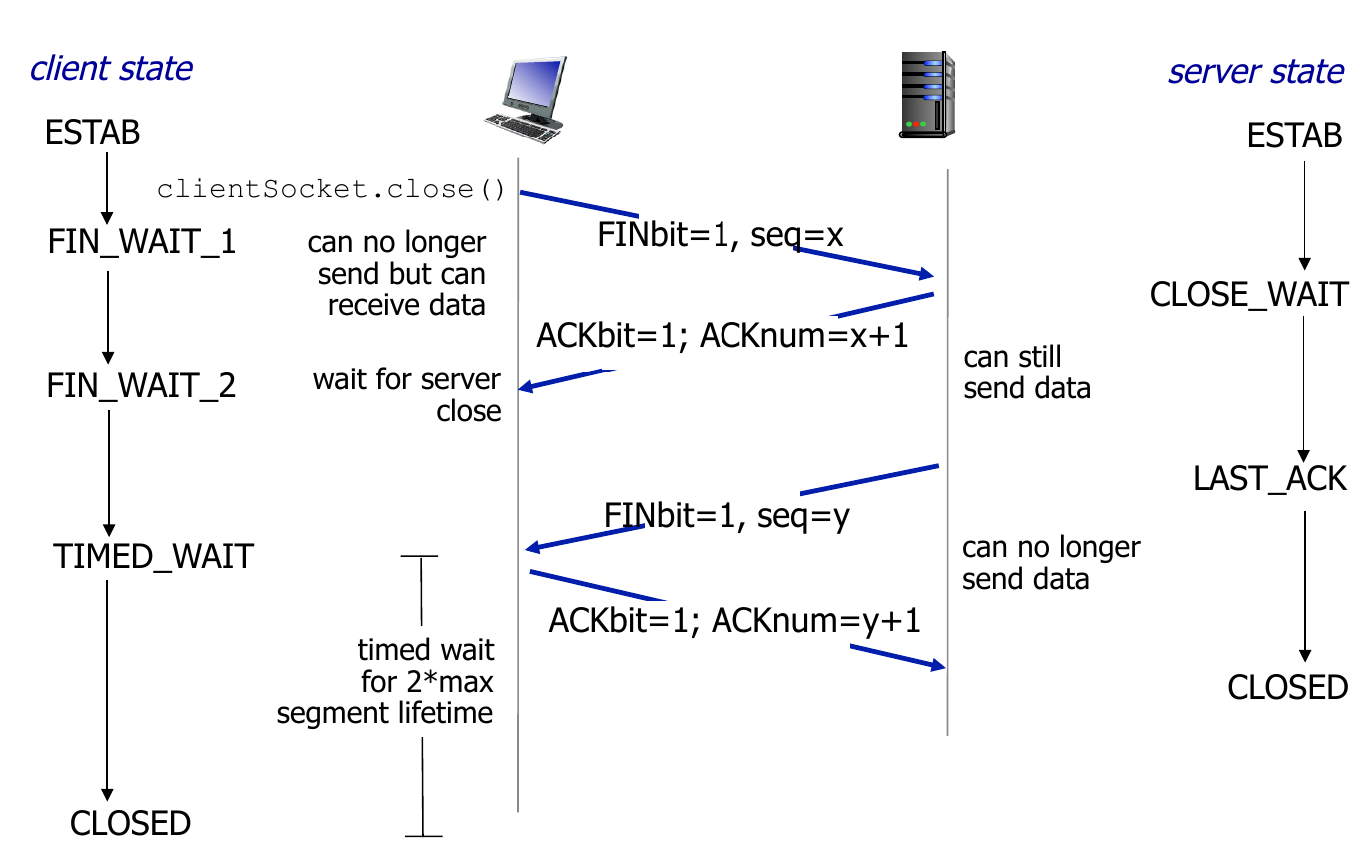
\includegraphics[width=\textwidth]{./img/chiusuraconnessionetcp.png}  

\subsection{Principi del controllo di congestione}
La \textbf{congestione} è il blocco della rete per via di un numero di dati elevato mandati a una velocità elevata che la \textit{rete} non riesce a gestirli. 
Ciò causa pacchetti smarriti (overflow nel buffer) e lunghi ritardi (di accodamento nei buffer). 

\subsubsection*{Scenario 1}

\subsubsection*{Scenario 2}
I buffer hanno dimensione \textit{finita}

\subsubsection*{Scenario 3}

\subsubsection*{Scenario 4}

\subsection{Controllo di congestione}
Bisogna limitare la trasmissione, si effettua mdiante una "finestra di congestione" (CongWin), cioè una funzione dinamina della congestione. 
\[\text{Frequenza d'invio} = \frac{\text{CongWin}}{\text{RTT}} \text{byte/sec}\] 
Definiamola come una misura a spanne, non precisa. \\

Il mittente si accorge della congestione tramite il \textit{timeout} o il \textit{triplice ACK duplicato}.
Il mittente riduce la \textit{frequenza d'invio} dopo essersi accorto, con tre meccanismi:
\begin{enumerate}
  \item \textbf{Partenza lenta}: Stabilita la connessione si manda un solo pacchetto. All'inizio la velocità di trasmissione è molto lenta, poi crescerà a livello esponenziale finché non si verifica un evento di perdita, raddoppiamo la \textit{finestra di congestione} dopo ogni \textit{RTT} (ogni volta che torna un \textit{ACK}). La \textit{partenza lenta} progredisce fino a un valore di soglia deciso dai progettisti. \\ 
    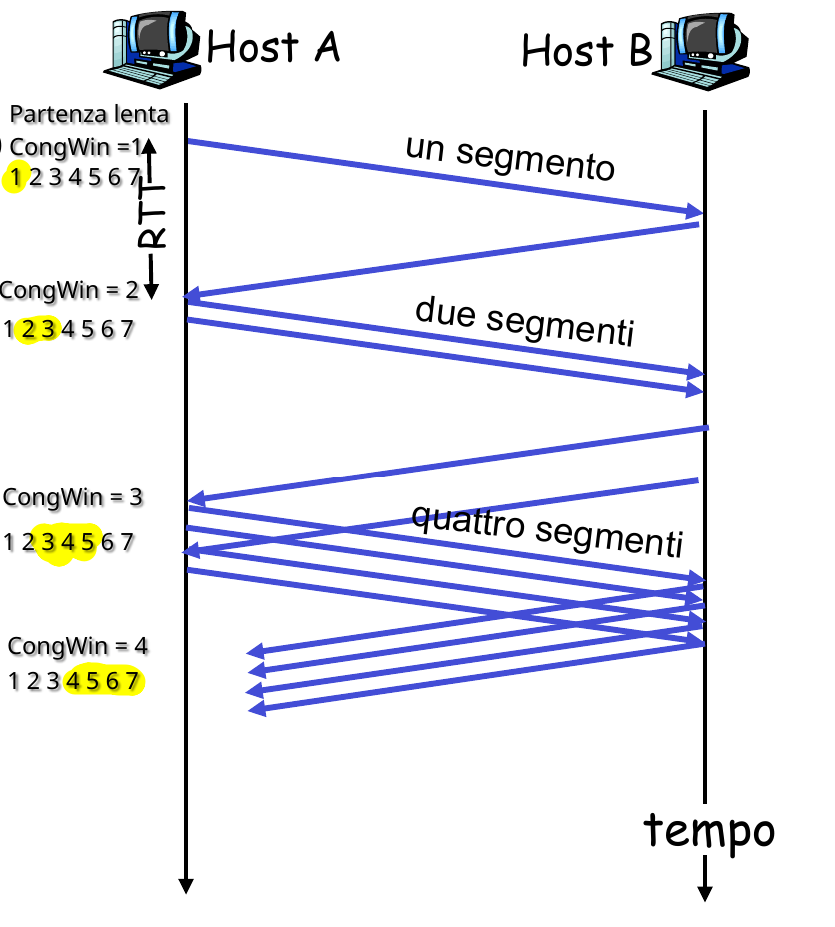
\includegraphics[width=\textwidth]{./img/partenzalenta.png} \\
    Nel caso di \textit{triplice ACK duplicato} si passa all'algoritmo successivo per una crescita più lenta, impostando però:
    \[\text{valore di soglia} = \frac{\text{CongWin}}{2}\]
    \[\text{CongWin} = \text{valore di soglia}\]
  \item \textbf{AIMD}: Incremento additivo, decremento moltiplicativo in italiano. \textbf{Fase a regime}, dopo la partenza lenta. La crescita della \textit{finestra} continua in maniera lineare di \textbf{1 MSS} dopo ogni \textit{RTT}, nel caso di errori la \textit{finestra} viene \textbf{dimezzata}. Questo è il suo andamento: \\
    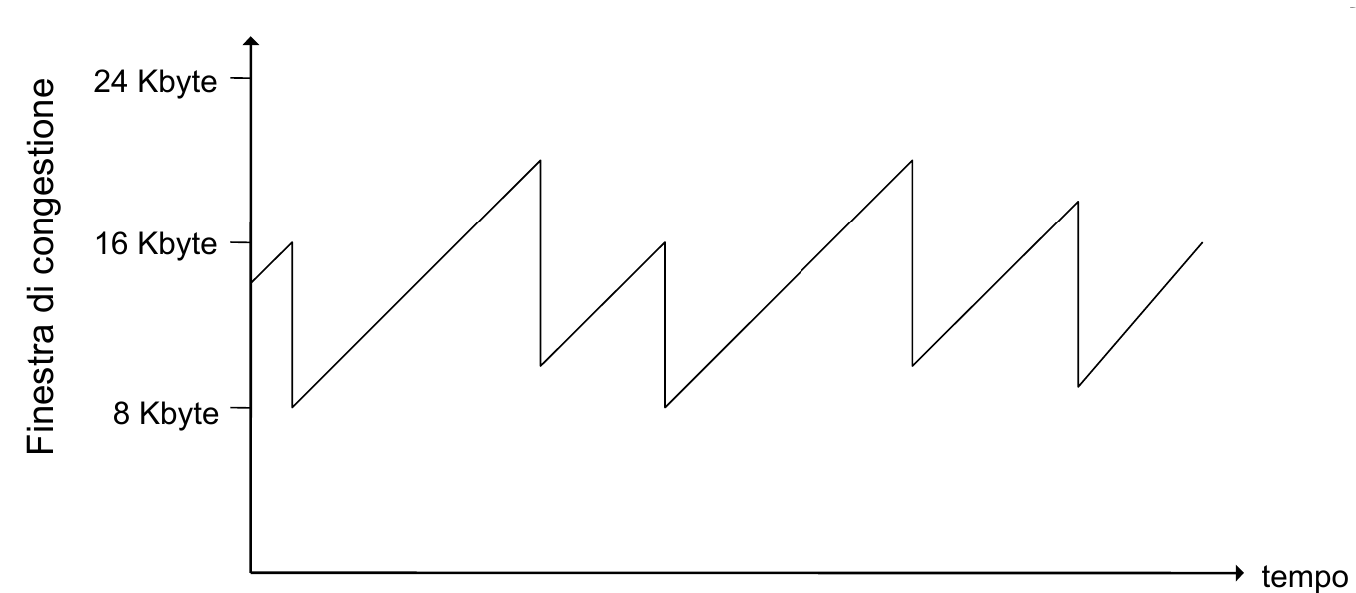
\includegraphics[width=\textwidth]{./img/AIMD.png} \\ 
    Il suo funzionamento è così diagrammato: \\ 
    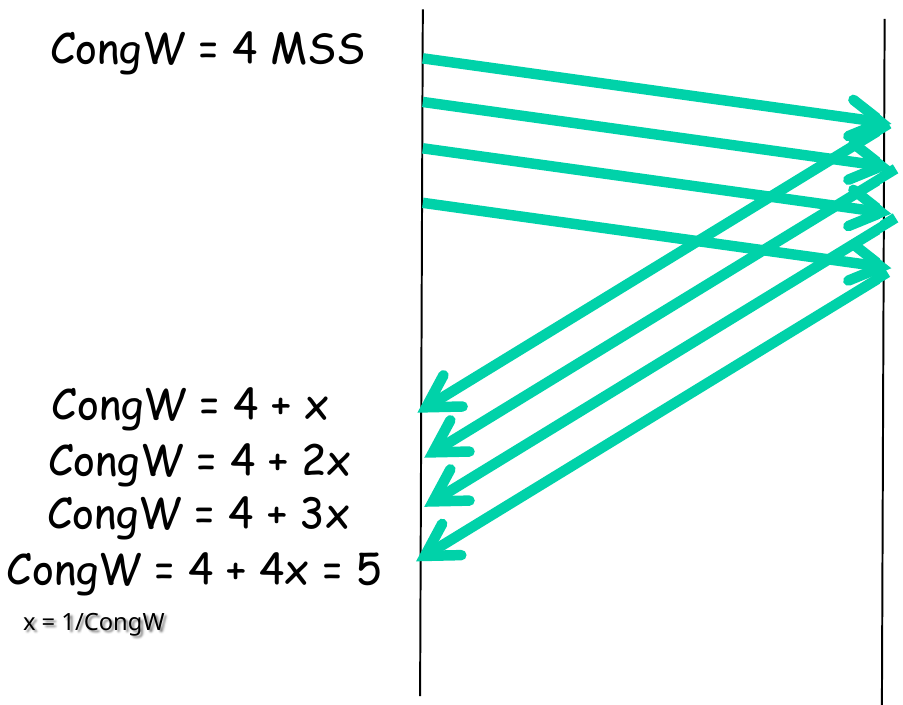
\includegraphics[width=\textwidth]{./img/AIMD-2.png} \\ 
    negli esercizi, in caso di perdita di \textit{ACK}, arrotondiamo a +1 la frazione, solo per comodità. Nella realtà, essendo in byte, si fa il calcolo e si mantiene quel valore, non ci sono problemi in caso di perdità di ACK poiché l'ACK cumulativo conferma pure il pacchetto perso.
  \item \textbf{Reazione agli eventi di perdita}: Dividiamo i casi. Nel caso in cui si verifica il \textit{timeout} resettiamo la \textit{finestra} a 1, tornando così alla \textit{partenza lenta}, il valore di soglia viene impostato a 
    \[\text{Valore di soglia} = \frac{\text{CongWin}}{2} \]
    \[\text{CongWin} = 1\] \\ 
    Nel caso in cui abbaimo una perdita (\textbf{Fast recovery}), \textit{triplice ACK duplicato}, imposto 
    \[\text{CongWin} = \frac{\text{CongWin}}{2} \]
    \[\text{Valore di soglia} = \text{CongWin}\]
\end{enumerate}

\subsubsection*{Diagramma riassuntivo}
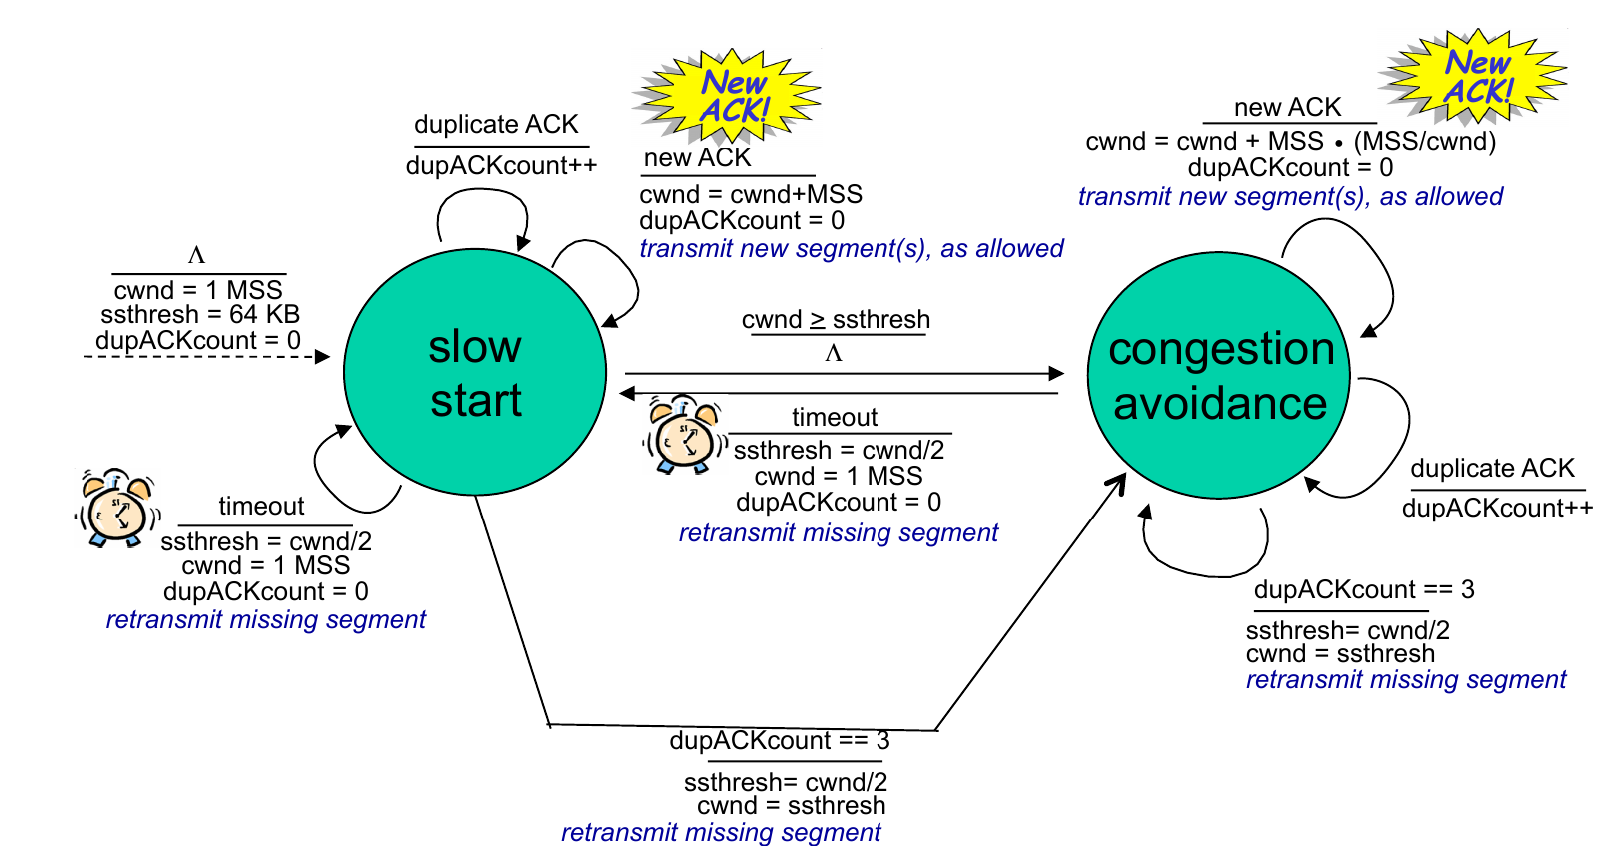
\includegraphics[width=\textwidth]{./img/diagrammacontrollodicongestione.png} \\

\subsubsection{Throughput TCP}

\subsection{Programmazione delle socket}
Le \textbf{socket} mettono in comunicazione \textit{livello applicativo} con il \textit{livello di trasporto}. 
Esistono due tipi di \textit{socket}: \textbf{UDP} e \textbf{TCP}. 

Il \textit{server} crea una socket col comando \texttt{socket()}, inizialmente crea la \texttt{socket di benvenuto}, quindi si crea una \textit{socket} senza parametri, bisogna comunicarglieli successivament.
Il \textit{server} aggancia i parametri alla \textit{socket} precedentemente creata tramite il comando \texttt{bind()}. Mettiamo il \textit{server} in stato di ascolto tramite il comando \texttt{listen()}. 

Il \textit{client} crea una socket con i parametri del \textit{server}, tramite il comando \texttt{socket()}. 
Il \textit{client} aggancia i 4 parametri alla \textit{socket} precedentemente creata con il comando \texttt{bind()}. 
Il \textit{client} si connette al server mediante il comando \texttt{connect()}, il \textit{server} dall'altra parte accetterà la connessione sulla \textit{socket specifica} col comando \texttt{accept()}, e manda il messaggio \textbf{SYNACK}.
Il \textit{client} manda il messaggio al \textit{server} mediante il comando \texttt{send()} che verrà ricevuto dal comando \texttt{recv()} dal \textit{server}, mandando in risposta tramite \texttt{send()} l'\textbf{ACK}, che verrà ricevuto dal \textit{client} tramite \texttt{recv()}. 

Si usa il comando \texttt{close()} per chiudere la connessione, possono mandarlo sia \textit{server} che \textit{client}, mandando il messaggio di \textbf{FIN}, ricevendo in risposta un \textbf{FINACK}. 

\subsubsection*{\texttt{socket()}}
Creazione della \textit{socket}: \texttt{int s\_listen = socket(family, type, protocol);} \\ 
family: AF\_INET specifica IPV4 \\ type: SOCK\_STREAM, SOCK\_DGRAM \\ protocol: 0 (pseudo, IP). \\
Avremo un identificativo della socket come ritorno della funzione. 

\subsubsection*{\texttt{bind()}}
Aggancio dei parametri alla \textit{socket} precedentemente creata vuota: \\ 
\texttt{bind(s\_listen = localAdd, AddLength);} \\
Si specifica la porta su cui mettersi in ascolto. \\ 
s\_listen: identificatore della \textit{socket} \\ 
localAdd: di tipo \textbf{sockaddr\_in}, una struttura già definita. \\ 
AddLength: lunghezza della variabile localAdd \\ 
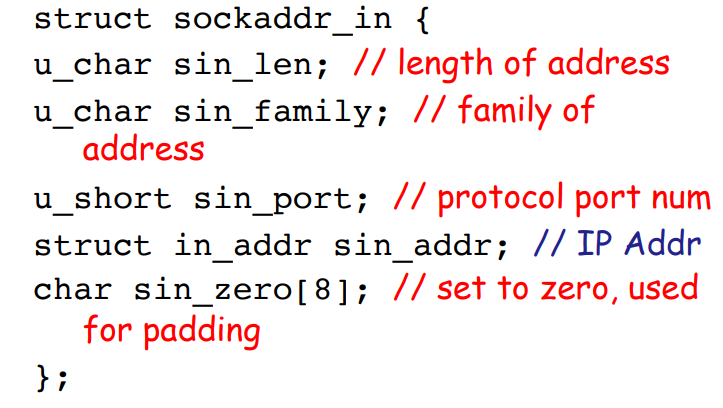
\includegraphics[width=\textwidth]{./img/struct_sockaddr_In.png} \\

Definisco \texttt{struct sockaddr\_in sockAdd;}
Imposto la famiglia: \texttt{sockAdd.sin\_family = AF\_INET;}
Per impostare l'indirizzo IPV4 abbiamo due modi:
\begin{enumerate}
  \item Specifichiamo l'indirizzo da ascoltare: \texttt{inet\_pton(AF\_INET, “127.0.0.1”, \&sockAdd.sin\_addr.s\_addr);}
  \item Ascolta da tutti gli indirizzi locali (in questo caso): \texttt{sockAdd.sin\_addr.s\_addr = htonl(INADDR\_ANY);}
\end{enumerate}
Imposto la porta: \texttt{sockAdd.sin\_port = htons(9999);}

\subsubsection*{\texttt{listen()}}
\texttt{int status = listen(s\_listen, queuelength);} \\ 
Risultato: -1 errore, 0 ok \\ 
s\_listen: riferimento alla socket \\ 
queuelength: numero di client che possono stare in attesa. \\ 
È una funzione \textbf{non bloccante}, ritorna immediatamente un valore. 

\subsubsection*{\texttt{accept()}}
\texttt{int s\_new = accept(s\_listen, \&clientAddress, \&AddLength);}
s\_new: nuova socket per la comucazione con il client, fino ad adesso abbiamo usato una \textit{socket di benvenuto}. \\ 
s\_listen: riferimento alla vecchia socket di benvenuto \\ 
clientAddress: riferimento alla struttura sockAddr\_in con l'indirizzo del client. \\ 
AddLength: dimensione della variabile clientAddress. \\ 
È una funzione \textbf{bloccante}, ritorna un valore solo quando riceve una richiesta di connessione. 

\subsubsection*{\texttt{send()}}
\texttt{int send(int s\_new, const void *buf, int len, int flags);}
s\_new: descrittore della socket \\ 
buf: puntatore al buffer \\ 
len: dimensione del buffer \\ 
flags: da impostare a 0 

\subsubsection*{\texttt{recv()}}
\texttt{int recv(int s\_new, void *buf, int len, unsigned int flags);}
Simile alla send \\ 
buf: conterrà i dati da ricevere 

\subsubsection*{\texttt{fork()}}
Funzione della libreria di C, \textbf{biforca} il \textit{processo}, creando \textbf{processo padre} e \textbf{processo figlio}, processi identici con stesse variabili. Il \textit{processo figlio} gestirà le connessioni con il \textit{client} mentre col \textit{processo padre} gestiamo il \textit{listening}, rimandendo in \texttt{accept()}, ogni volta che gli arriverà una nuova richiesta per una socket faremo il \texttt{fork()} del processo padre, affidando al figlio la socket appena creata.

